% !TEX root = ../thesis-example.tex
%
\chapter{Extraction d'Information sur les Demandes}
\label{sec:quanta}

\section{Introduction}
\label{sec:quanta:introduction}
Au coeur de l'analyse des décisions de justice se trouve le concept de demande. Il s'agit d'une réclammation ou requête effectuée par une des parties devant le juge. Par exemple, une partie peut demander des dommages-intérêts en réparation d'un préjudice subi, ou bien un divorce, ou bien des indemnités auxquelles elle pense avoir droit, ou encore un simple constat ... Les demandes sont fondamentales car l'argumentation durant le déroulement de l'affaire n'a qu'un seul but : faire accepter ses demandes et faire rejetter celle de la partie adverse. L'extraction des demandes et des résultats correspondant, dans un corpus, permet ainsi d'avoir une estimation quantifiée de la décision des juges sur des types de demandes. Les informations qui nous intéressent sont la \textbf{catégorie de la demande}, le \textbf{quantum ou montant demandé}, le \textbf{sens du résultat} (la demande a-t-elle été acceptée ou rejettée?), et le \textbf{quantum ou montant obtenu} (décidé par les juges). Pour pouvoir extraire les demandes et les résultats, il est nécessaire de comprendre comment ils sont exprimés et coreférencés dans les décisions jurisprudentielles. Leur expression peut comporter plus ou moins de complexité avec souvent des références à des jugements antérieurs, des agrégations ou des restrictions (Figure \ref{fig:quanta:expr-dmd-rst}).

\begin{figure}[h]
\scriptsize
\begin{subfigure}[t]{0.9\textwidth}
\fbox{\parbox{\textwidth}{Jennifer M., Catherine M. et Sandra M. ... demandent à la Cour de :

- les recevoir régulièrement appelantes incidentes du \textcolor{blue}{jugement du 23/05/2014} ;

- infirmer \textcolor{blue}{le dit jugement} en \textcolor{brown}{toutes ses dispositions} ; ...

Statuant à nouveau ...

- \textcolor{brown}{les condamner au paiement d'une somme de  3 000,00 \euro{} pour procédure abusive et aux entiers dépens} ; }}
\caption{Exemples d'expression de demandes}\label{fig:quanta:expr-dmd}
\end{subfigure} 


\begin{subfigure}[t]{0.9\textwidth}
\fbox{\parbox{\textwidth}{La cour, ...  


CONFIRME \textcolor{blue}{le jugement entreprise} en \textcolor{brown}{toutes ses dispositions}.

Y ajoutant

\textcolor{gray}{CONSTATE que Amélanie Gitane P. épouse M. est défaillante à rapporter la preuve
d'une occupation trentenaire lui permettant d'invoquer la prescription
acquisitive de la parcelle BH 377 située [...].}

\textcolor{gray}{DEBOUTE Amélanie Gitane P. épouse M. de sa demande en dommages et intérêts.}

\textcolor{gray}{CONDAMNE Amélanie Gitane P. épouse M. aux dépens d'appel.}

\textcolor{gray}{DIT n'y avoir lieu à l'application de l'article 700 du Code de Procédure Civile.}
}}
\caption{Exemple d'expression de résultat}\label{fig:quanta:expr-rst}
\end{subfigure}
\caption{Expressions \textcolor{gray}{simples}, ou comprenant des  \textcolor{blue}{références} et  des \textcolor{brown}{agrégations} (extraits de la décision 14/01082 de la cour d'appel de Saint-Denis (Réunion))}\label{fig:quanta:expr-dmd-rst}
\end{figure}

\subsection{Données cibles à extraire}
\subsubsection{Catégorie de demande}
Une catégorie de demande regroupe les prétentions qui sont de même nature par le fait qu'elles partagent deux aspects: l'\textbf{objet} demandé (par ex. dommages-intérêts, amende, déclaration de créance, ...) et le fondement c'est-à-dire les règles ou normes ou principes juridiques qui fondent la demande (par ex. article 700 du code de procédure civile). Des expressions particulières sont souvent utilisées pour faire référence aux catégories (Tableau \ref{tab:quanta:exemple-categorie}).

\begin{table}[h!]
\scriptsize
\begin{tabular}{|p{0.45\textwidth}|p{0.15\textwidth}|p{0.3\textwidth}|}
\hline
\textbf{Expression nominative  }                                     & \textbf{Objet}                                                       & \textbf{Normes}                                                                 \\ \hline
dommages-intérêts pour abus de procédure                    & dommages-intérêts                                           & Articles 32-1 code de procédure civile + 1382 code de procédure civile \\ \hline
amende civile pour abus de procédure                        & amende civile                                               & Articles 32-1 code de procédure civile + 559 code de procédure civile  \\ \hline
frais irrépétibles                                          & dommages-intérêts                                           & Article 700 du code de procédure civle                                 \\ \hline
dommages-intérêts pour trouble de voisinage                 & dommages-intérêts                                           & principe de responsabilité pour trouble anormal de voisinage           \\ \hline
déclaration de créance au passif de la procédure collective & déclaration de créance & L622-24 code de commerce                                               \\ \hline
dommages-intérêts pour concurence déloyale                  & dommages-intérêts                                           & Article 1382 du code civil                                             \\ \hline
\end{tabular}
\caption{Exemples de catégories de demandes}\label{tab:quanta:exemple-categorie}
\end{table}

\subsubsection{Quantum demandé}
Le quantum demandé quantifie l'objet de la demande. Par exemple, dans l'exemple de la Figure \ref{fig:quanta:expr-dmd}, "3000 \euro{}" est le quantum demandé pour dommages-intérêts pour procédure abusive. Bien que, dans cette étude, nous ne nous intéressons particulièrement qu'aux montants d'argent, le quantum peut être une durée (garde d'enfant, ou emprisonement, ...). Toutes les catégories demandes n'ont pas un quantum (par ex. une demande de divorce) et seul le sens du résultat sera la données à extraire dans ce cas.

\subsubsection{Sens du résultat}
Le sens du résultat est l'interprétation de la réponse des juges à une demande. En général, le sens peut être positif si la demande a été \textbf{acceptée} ou négatif si la demande a été \textbf{rejetée}. Il arrive aussi que le résultat soit reporté à un jugement futur (un \textbf{sursis à statuer} est alors prononcé). 

\subsubsection{Quantum obtenu ou quantum résultat}
Le quantum obtenu quantifie le résultat ou la réponse des juges. Il est en général inférieur ou égal au quantum demandé. Si la demande est rejetée, le quantum est évidemment nul. il doit être de la même nature que le quantum demandé (montant d'argent ou durée).

\subsection{Expression, défis et indicateurs d'extraction}
Les demandes sont décrites à la fin de la section d'exposé des faits, procédures, moyens et prétentions des parties (section LITIGE). Elles rentrent donc dans les "moyens et prétentions des parties" qui regroupent les demandes et les arguments des parties. Quant aux résultats, ils sont décrits dans la section DISPOSITIF et dans la section MOTIFS (raisonnement des juges). Les demandes sont exprimées en paragraphe où chaque paragraphe correspond soit à une partie, soit à un groupe de partie partageant les mêmes demandes (par ex. des époux). Le paragraphe est parfois organisé en liste dont chaque élément exprime une ou plusieurs demandes, ou fait référence à un jugement antérieur. Les résultats ont aussi la forme de liste dans la section DISPOSITIF. Par contre, dans les motifs de la décision, les raisonnements sont organisés en paragraphes, et ordonnés catégorie après catégorie. Le résultat est donné à la fin du groupe de paragraphes associé à la catégorie. Cette pseudo-structure n'est pas standard et elle impose de nombreux défis à relever.

D'une part, la séparation des demandes et des résultats rend difficile la résolution de coréférence entre prétentions et résultats. En effet, un décision jurisprudentielle porte sur plusieurs demandes pour lesquelles il faut identifier le quantum demandé, le sens du résultat et le quantum obtenu. il est important de faire correspondre un quantum demandé extrait au sens et au quantum du résultat qui font référence à la même demande. D'autre part, les références aux jugements antérieurs exigent de résoudre des références aux résultats de jugements antérieurs qui sont, heureusement, rappelés dans le même document. \textbf{agrégations, redondances dans les jugements et demandes, et dans les motifs etle dispositifs, la non structuration ou non standardisation des documents pas évident une mth à base de règles, grand nombre de catégories => difficile d'annoter suffisamment de données}.

Le vocabulaire utilisé est très souvent lié à des types de demandes et réciproquement, ce vocabulaire permet de rapprocher des demandes de même nature dans des catégories. Par exemple le dernier élément de la Fig. \ref{fig:quanta:expr-dmd} comprend le terme "\textit{pour procédure abusive}" qui est près d'une somme d'argent (\textit{3000 \euro{}}); il est donc probable que ce type de terme assez particulier soit un bon indicateur de la position des quanta. Par ailleurs, des verbes particuliers sont utilisés pour exprimer les prétentions et résultats : infirmer, confirmer, cosntater, débouter, dire, ... Ce sont d'autres indicateurs qui peuvent être exploités implicitement ou explicitement. Comme autres formes récurrentes, on pourrait citer l'ordre des demandes (resp. résultats). Généralement, on a les constats, les références aux jugements antérieurs, les demandes principales (?) et secondaires (?).

\section{Formulation du problème}
\label{sec:quanta:probleme}

\section{Synthèse bibliographique associée}
\label{sec:quanta:biblio}

\section{Méthode1: Localisation à Base d'Expressions clés prédéfinies et Apprises Automatiquement}
\label{sec:quanta:baseline}

\subsection{Sélection des termes clés de la catégories: ngram2vec > cluster de ngram > sélection des clusters associés à la catégorie }

\url{https://github.com/azpoliak/eco}

\section{Méthode2: Chaine d'extraction à base de classification}

\section{Méthode3: Extraction par prédiction structurée}

\section{Expérimentations et interprétation des résultats}
\label{sec:quanta:xp}

\subsection{Annotation de données d'évaluation}
\label{sec:quanta:xp:dataset}
\begin{figure}
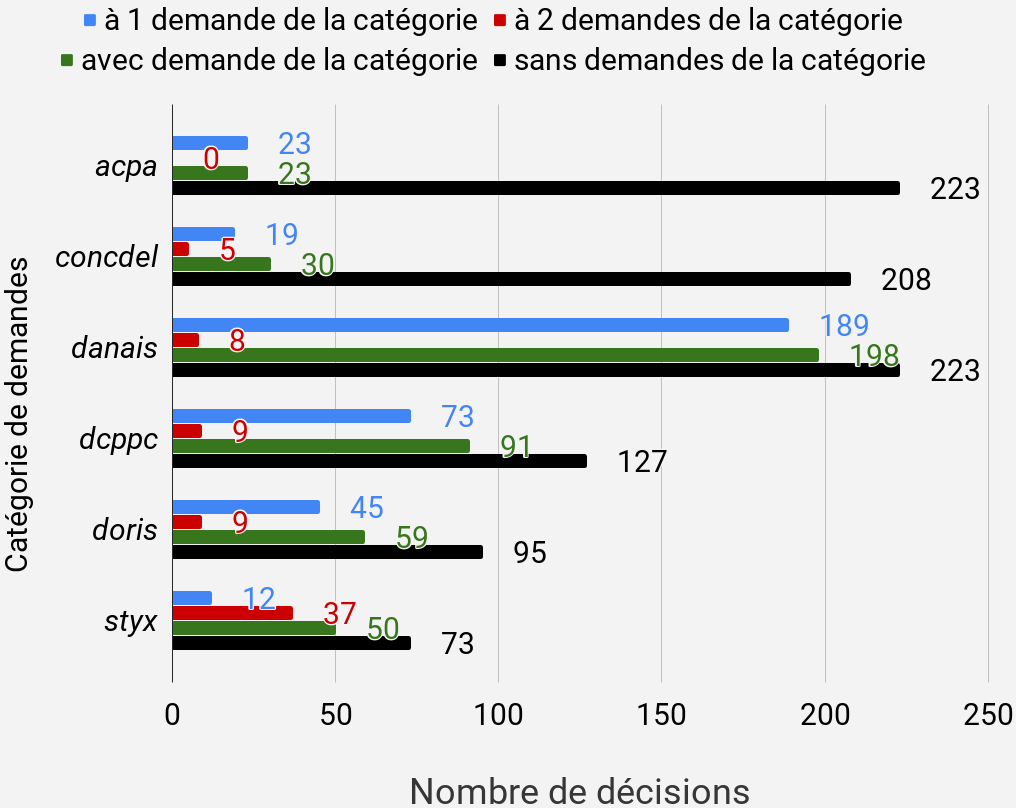
\includegraphics[width=\textwidth]{chartDataset.png}
\caption{Répartitions des demandes dans les documents annotées pour chaque catégorie.}\label{stat-alldata-dmd}
\end{figure}

\subsection{Métriques d'évaluation}
\label{sec:quanta:xp:metrics}
% \begin{figure}[htb]
% 	\includegraphics[width=\textwidth]{gfx/Clean-Thesis-Figure}
% 	\caption{Figure example: \textit{(a)} example part one, \textit{(c)} example part two; \textit{(c)} example part three}
% 	\label{fig:system:example1}
% \end{figure}

\subsection{Cas des décisions à une demande}

\subsection{Cas général}

\section{Conclusion}
\label{sec:quanta:conclusion}

